\documentclass[twoside]{book}

% Packages required by doxygen
\usepackage{calc}
\usepackage{doxygen}
\usepackage{graphicx}
\usepackage[utf8]{inputenc}
\usepackage{makeidx}
\usepackage{multicol}
\usepackage{multirow}
\usepackage{textcomp}
\usepackage[table]{xcolor}

% Font selection
\usepackage[T1]{fontenc}
\usepackage{mathptmx}
\usepackage[scaled=.90]{helvet}
\usepackage{courier}
\usepackage{amssymb}
\usepackage{sectsty}
\renewcommand{\familydefault}{\sfdefault}
\allsectionsfont{%
  \fontseries{bc}\selectfont%
  \color{darkgray}%
}
\renewcommand{\DoxyLabelFont}{%
  \fontseries{bc}\selectfont%
  \color{darkgray}%
}

% Page & text layout
\usepackage{geometry}
\geometry{%
  a4paper,%
  top=2.5cm,%
  bottom=2.5cm,%
  left=2.5cm,%
  right=2.5cm%
}
\tolerance=750
\hfuzz=15pt
\hbadness=750
\setlength{\emergencystretch}{15pt}
\setlength{\parindent}{0cm}
\setlength{\parskip}{0.2cm}
\makeatletter
\renewcommand{\paragraph}{%
  \@startsection{paragraph}{4}{0ex}{-1.0ex}{1.0ex}{%
    \normalfont\normalsize\bfseries\SS@parafont%
  }%
}
\renewcommand{\subparagraph}{%
  \@startsection{subparagraph}{5}{0ex}{-1.0ex}{1.0ex}{%
    \normalfont\normalsize\bfseries\SS@subparafont%
  }%
}
\makeatother

% Headers & footers
\usepackage{fancyhdr}
\pagestyle{fancyplain}
\fancyhead[LE]{\fancyplain{}{\bfseries\thepage}}
\fancyhead[CE]{\fancyplain{}{}}
\fancyhead[RE]{\fancyplain{}{\bfseries\leftmark}}
\fancyhead[LO]{\fancyplain{}{\bfseries\rightmark}}
\fancyhead[CO]{\fancyplain{}{}}
\fancyhead[RO]{\fancyplain{}{\bfseries\thepage}}
\fancyfoot[LE]{\fancyplain{}{}}
\fancyfoot[CE]{\fancyplain{}{}}
\fancyfoot[RE]{\fancyplain{}{\bfseries\scriptsize Generated on Sun Mar 22 2015 17\-:51\-:17 for Boost.\-Document by Doxygen }}
\fancyfoot[LO]{\fancyplain{}{\bfseries\scriptsize Generated on Sun Mar 22 2015 17\-:51\-:17 for Boost.\-Document by Doxygen }}
\fancyfoot[CO]{\fancyplain{}{}}
\fancyfoot[RO]{\fancyplain{}{}}
\renewcommand{\footrulewidth}{0.4pt}
\renewcommand{\chaptermark}[1]{%
  \markboth{#1}{}%
}
\renewcommand{\sectionmark}[1]{%
  \markright{\thesection\ #1}%
}

% Indices & bibliography
\usepackage{natbib}
\usepackage[titles]{tocloft}
\setcounter{tocdepth}{3}
\setcounter{secnumdepth}{5}
\makeindex

% Hyperlinks (required, but should be loaded last)
\usepackage{ifpdf}
\ifpdf
  \usepackage[pdftex,pagebackref=true]{hyperref}
\else
  \usepackage[ps2pdf,pagebackref=true]{hyperref}
\fi
\hypersetup{%
  colorlinks=true,%
  linkcolor=blue,%
  citecolor=blue,%
  unicode%
}

% Custom commands
\newcommand{\clearemptydoublepage}{%
  \newpage{\pagestyle{empty}\cleardoublepage}%
}


%===== C O N T E N T S =====

\begin{document}

% Titlepage & ToC
\hypersetup{pageanchor=false}
\pagenumbering{roman}
\begin{titlepage}
\vspace*{7cm}
\begin{center}%
{\Large Boost.\-Document }\\
\vspace*{1cm}
{\large Generated by Doxygen 1.8.6}\\
\vspace*{0.5cm}
{\small Sun Mar 22 2015 17:51:17}\\
\end{center}
\end{titlepage}
\clearemptydoublepage
\tableofcontents
\clearemptydoublepage
\pagenumbering{arabic}
\hypersetup{pageanchor=true}

%--- Begin generated contents ---
\chapter{Hierarchical Index}
\section{Class Hierarchy}
This inheritance list is sorted roughly, but not completely, alphabetically\-:\begin{DoxyCompactList}
\item \contentsline{section}{boost\-:\-:document}{\pageref{classboost_1_1document}}{}
\item \contentsline{section}{boost\-:\-:document\-\_\-file\-\_\-format}{\pageref{structboost_1_1document__file__format}}{}
\item logic\-\_\-error\begin{DoxyCompactList}
\item \contentsline{section}{boost\-:\-:document\-\_\-exception}{\pageref{classboost_1_1document__exception}}{}
\end{DoxyCompactList}
\end{DoxyCompactList}

\chapter{Class Index}
\section{Class List}
Here are the classes, structs, unions and interfaces with brief descriptions\-:\begin{DoxyCompactList}
\item\contentsline{section}{\hyperlink{classboost_1_1document}{boost\-::document} }{\pageref{classboost_1_1document}}{}
\item\contentsline{section}{\hyperlink{classboost_1_1document__exception}{boost\-::document\-\_\-exception} }{\pageref{classboost_1_1document__exception}}{}
\item\contentsline{section}{\hyperlink{structboost_1_1document__file__format}{boost\-::document\-\_\-file\-\_\-format} }{\pageref{structboost_1_1document__file__format}}{}
\end{DoxyCompactList}

\chapter{Class Documentation}
\hypertarget{classboost_1_1document}{\section{boost\-:\-:document Class Reference}
\label{classboost_1_1document}\index{boost\-::document@{boost\-::document}}
}
\subsection*{Public Member Functions}
\begin{DoxyCompactItemize}
\item 
\hypertarget{classboost_1_1document_af1a85718219b8da6f1befaac0bf87989}{\hyperlink{classboost_1_1document_af1a85718219b8da6f1befaac0bf87989}{document} ()}\label{classboost_1_1document_af1a85718219b8da6f1befaac0bf87989}

\begin{DoxyCompactList}\small\item\em Default Constructor. Not preferred at all. \end{DoxyCompactList}\item 
\hypertarget{classboost_1_1document_a2c3bcea48dfd233e0255ae4dd274b6da}{\hyperlink{classboost_1_1document_a2c3bcea48dfd233e0255ae4dd274b6da}{document} (const boost\-::filesystem\-::path path)}\label{classboost_1_1document_a2c3bcea48dfd233e0255ae4dd274b6da}

\begin{DoxyCompactList}\small\item\em The de facto Constructor. Creates a new document object. \end{DoxyCompactList}\item 
\hypertarget{classboost_1_1document_afff6a78ede7767d8cbc0cb4566ae64da}{\hyperlink{classboost_1_1document_afff6a78ede7767d8cbc0cb4566ae64da}{$\sim$document} ()}\label{classboost_1_1document_afff6a78ede7767d8cbc0cb4566ae64da}

\begin{DoxyCompactList}\small\item\em Destructor Closes Unsaved Documents. \end{DoxyCompactList}\item 
\hypertarget{classboost_1_1document_a9e89218509ba65a56d088de9d4696cc5}{void \hyperlink{classboost_1_1document_a9e89218509ba65a56d088de9d4696cc5}{open\-\_\-document} ()}\label{classboost_1_1document_a9e89218509ba65a56d088de9d4696cc5}

\begin{DoxyCompactList}\small\item\em Opens document using Calc/\-Excel given in the file path. \end{DoxyCompactList}\item 
\hypertarget{classboost_1_1document_a3c6af22aa585c734aa8de19dc2b4b335}{void \hyperlink{classboost_1_1document_a3c6af22aa585c734aa8de19dc2b4b335}{open\-\_\-document} (const boost\-::filesystem\-::path \&path)}\label{classboost_1_1document_a3c6af22aa585c734aa8de19dc2b4b335}

\begin{DoxyCompactList}\small\item\em Opens document using Calc/\-Excel given in the file path. \end{DoxyCompactList}\item 
\hypertarget{classboost_1_1document_a8b5fa1ec18c56babaa03739ebe363359}{void \hyperlink{classboost_1_1document_a8b5fa1ec18c56babaa03739ebe363359}{close\-\_\-document} ()}\label{classboost_1_1document_a8b5fa1ec18c56babaa03739ebe363359}

\begin{DoxyCompactList}\small\item\em Closes document using Calc/\-Excel given in the file path. \end{DoxyCompactList}\item 
\hypertarget{classboost_1_1document_ae6fb37bb361f16b03090b4aa5221a869}{void \hyperlink{classboost_1_1document_ae6fb37bb361f16b03090b4aa5221a869}{close\-\_\-document} (const boost\-::filesystem\-::path \&path)}\label{classboost_1_1document_ae6fb37bb361f16b03090b4aa5221a869}

\begin{DoxyCompactList}\small\item\em Closes document using Calc/\-Excel given in the file path. \end{DoxyCompactList}\item 
\hypertarget{classboost_1_1document_a5523760f4758f1d45632d00d8c997c98}{void \hyperlink{classboost_1_1document_a5523760f4758f1d45632d00d8c997c98}{save\-\_\-document} ()}\label{classboost_1_1document_a5523760f4758f1d45632d00d8c997c98}

\begin{DoxyCompactList}\small\item\em saves document using Calc/\-Excel given in the file path. \end{DoxyCompactList}\item 
\hypertarget{classboost_1_1document_acad48dd9e10a0e56b102003ddedc046e}{void \hyperlink{classboost_1_1document_acad48dd9e10a0e56b102003ddedc046e}{export\-\_\-document} (const boost\-::filesystem\-::path \&path, boost\-::document\-\_\-file\-\_\-format\-::type format=document\-\_\-file\-\_\-format\-::\-P\-D\-F)}\label{classboost_1_1document_acad48dd9e10a0e56b102003ddedc046e}

\begin{DoxyCompactList}\small\item\em Exports document using Calc/\-Excel given in the file path and the file format. Default format is P\-D\-F. \end{DoxyCompactList}\item 
\hypertarget{classboost_1_1document_adfb85f51a85f221a428a6d2fc87e13d4}{void \hyperlink{classboost_1_1document_adfb85f51a85f221a428a6d2fc87e13d4}{export\-\_\-document} (boost\-::document\-\_\-file\-\_\-format\-::type format=document\-\_\-file\-\_\-format\-::\-P\-D\-F)}\label{classboost_1_1document_adfb85f51a85f221a428a6d2fc87e13d4}

\begin{DoxyCompactList}\small\item\em Exports document using Calc/\-Excel given in the file path and the file format. Default format is P\-D\-F. \end{DoxyCompactList}\end{DoxyCompactItemize}


The documentation for this class was generated from the following files\-:\begin{DoxyCompactItemize}
\item 
include/boost/document/document.\-hpp\item 
src/document.\-cpp\end{DoxyCompactItemize}

\hypertarget{classboost_1_1document__exception}{\section{boost\-:\-:document\-\_\-exception Class Reference}
\label{classboost_1_1document__exception}\index{boost\-::document\-\_\-exception@{boost\-::document\-\_\-exception}}
}
Inheritance diagram for boost\-:\-:document\-\_\-exception\-:\begin{figure}[H]
\begin{center}
\leavevmode
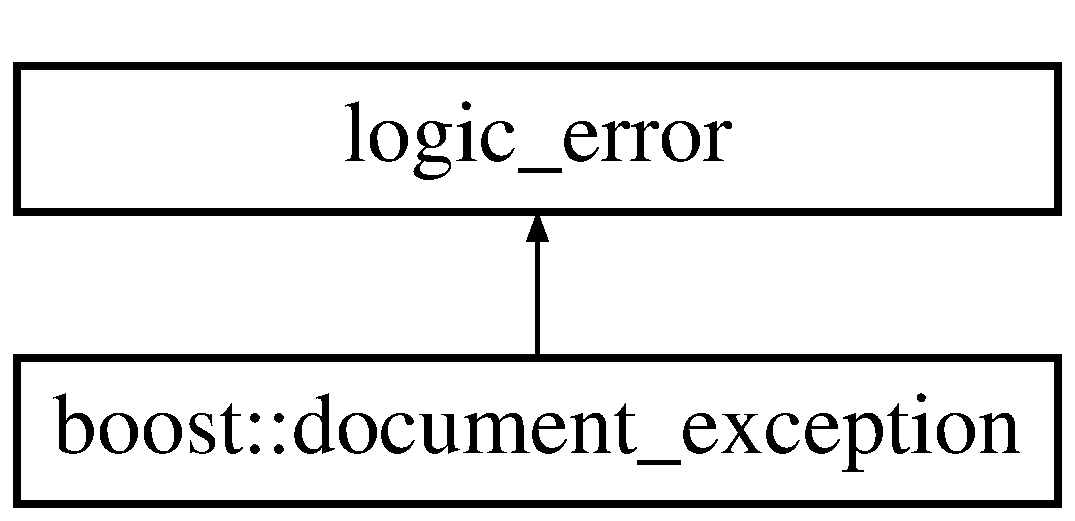
\includegraphics[height=2.000000cm]{classboost_1_1document__exception}
\end{center}
\end{figure}
\subsection*{Public Member Functions}
\begin{DoxyCompactItemize}
\item 
\hypertarget{classboost_1_1document__exception_aae571005033f3ba74b347294d5ddf495}{{\bfseries document\-\_\-exception} (const std\-::string \&msg)}\label{classboost_1_1document__exception_aae571005033f3ba74b347294d5ddf495}

\end{DoxyCompactItemize}


The documentation for this class was generated from the following file\-:\begin{DoxyCompactItemize}
\item 
include/boost/document/detail/document\-\_\-exception.\-hpp\end{DoxyCompactItemize}

\hypertarget{structboost_1_1document__file__format}{\section{boost\-:\-:document\-\_\-file\-\_\-format Struct Reference}
\label{structboost_1_1document__file__format}\index{boost\-::document\-\_\-file\-\_\-format@{boost\-::document\-\_\-file\-\_\-format}}
}
\subsection*{Public Types}
\begin{DoxyCompactItemize}
\item 
enum {\bfseries type} \{ {\bfseries P\-D\-F}, 
{\bfseries C\-S\-V}
 \}
\end{DoxyCompactItemize}


The documentation for this struct was generated from the following file\-:\begin{DoxyCompactItemize}
\item 
include/boost/document/detail/document\-\_\-file\-\_\-format.\-hpp\end{DoxyCompactItemize}

%--- End generated contents ---

% Index
\newpage
\phantomsection
\addcontentsline{toc}{chapter}{Index}
\printindex

\end{document}
